% Metódy inžinierskej práce

\documentclass[10pt,twoside,English,a4paper]{article}

\usepackage[english]{babel}
%\usepackage[T1]{fontenc}
\usepackage[IL2]{fontenc} % lepšia sadzba písmena Ľ než v T1
\usepackage[utf8]{inputenc}
\usepackage{booktabs} 
\usepackage{caption} 
\usepackage{subcaption} 
\usepackage{tikz}
\usepackage{array, hhline}
\usepackage{graphicx}
\usepackage{url} % príkaz \url na formátovanie URL
\usepackage{hyperref} % odkazy v texte budú aktívne (pri niektorých triedach dokumentov spôsobuje posun textu)
\usepackage{cite}
%\usepackage{times}

\pagestyle{headings}

\title{Real-time data processing in autonomous vehicles\thanks{Semestrálny projekt v predmete Metódy inžinierskej práce, ak. rok 2023/24, vedenie: Pavol Baťalík}} % meno a priezvisko vyučujúceho na cvičeniach

\author{Maksim Alehash\\[2pt]
	{\small Slovenská technická univerzita v Bratislave}\\
	{\small Fakulta informatiky a informačných technológií}\\
	{\small \texttt{xalehash@stuba.sk}}
	}

\date{\small \today} % upravte

\begin{document}

\maketitle

\tableofcontents


\begin{abstract}

\end{abstract}


\section{Introduction}

Motivujte čitateľa a vysvetlite, o čom píšete. Úvod sa väčšinou nedelí na časti.

Uveďte explicitne štruktúru článku. Tu je nejaký príklad.
Základný problém, ktorý bol naznačený v úvode, je podrobnejšie vysvetlený v časti~\ref{nejaka}.
Dôležité súvislosti sú uvedené v častiach~\ref{dolezita} a~\ref{dolezitejsia}.
Záverečné poznámky prináša časť~\ref{zaver}.



\section{Sensors and data sources} \label{nejaka}

Z obr.~\ref{f:rozhod} je všetko jasné. 

\begin{figure*}[tbh]
%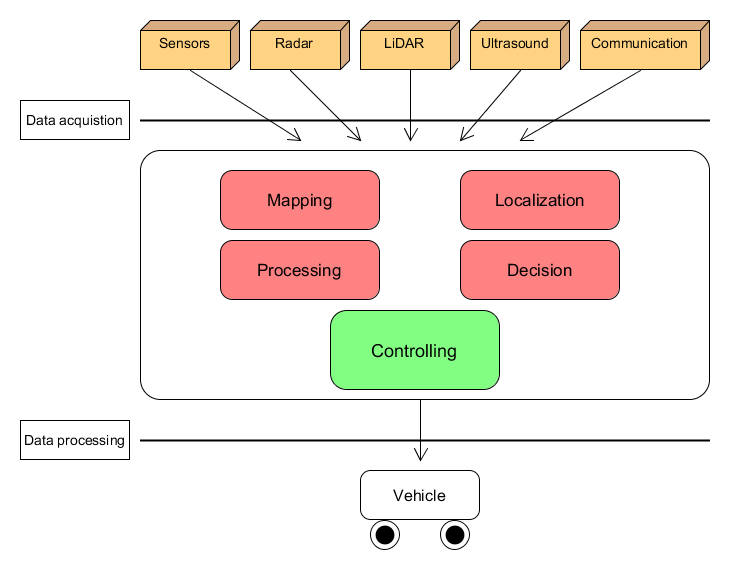
\includegraphics[scale=1.0]{diagram.pdf}
Aj text môže byť prezentovaný ako obrázok. Stane sa z neho označný plávajúci objekt. Po vytvorení diagramu zrušte znak \texttt{\%} pred príkazom \verb|\includegraphics| označte tento riadok ako komentár (tiež pomocou znaku \texttt{\%}).
\caption{Rozhodujúci argument.}
\label{f:rozhod}
\end{figure*}



\section{Data processing architecture} \label{ina}

Základným problémom je teda\ldots{} Najprv sa pozrieme na nejaké vysvetlenie (časť~\ref{ina:nejake}), a potom na ešte nejaké (časť~\ref{ina:nejake}).\footnote{Niekedy môžete potrebovať aj poznámku pod čiarou.}

Môže sa zdať, že problém vlastne nejestvuje\cite{Coplien:MPD}, ale bolo dokázané, že to tak nie je~\cite{Czarnecki:Staged, Czarnecki:Progress}. Napriek tomu, aj dnes na webe narazíme na všelijaké pochybné názory\cite{PLP-Framework}. Dôležité veci možno \emph{zdôrazniť kurzívou}.



\section{Algorithms and methods} \label{dolezita}




\section{Safety and performance} \label{dolezitejsia}




\section{Future directions and challenges} \label{dolezitejsia}




\section{Conclusion} \label{zaver} % prípadne iný variant názvu



%\acknowledgement{Ak niekomu chcete poďakovať\ldots}


% týmto sa generuje zoznam literatúry z obsahu súboru literatura.bib podľa toho, na čo sa v článku odkazujete
\bibliography{literatura}
\bibliographystyle{abbrv} % prípadne alpha, abbrv alebo hociktorý iný
\end{document}


